\chapter{Conexión local con la BD por defecto} \label{cap:03ConexLocal}

Generalmente, resulta de interés acceder a la base de datos remota de Broadsea desde un administrador de bases de datos local.  Docker almacena la base de datos de Broadsea en el volumen \code{atlasdb-postgres-data} (véase \ref{sec:01Docker} ''Entorno Docker de Broadsea'') y crea un entorno de interoperabilidad e interconectividad a través de la WebAPI, que se aloja en un servidor Postgre (véase \ref{sec:01Postgre} ''Entorno PostgreSQL de Broadsea'').

Por tanto, para acceder a la base de datos de ATLAS Broadsea se requiere acceder al servidor remoto de Broadsea, alojado en el \code{127.0.0.1} (véase \ref{cap:02Despliegue} ''Despliegue por defecto''), desde la instancia local de Postgres. La información relevante para esta implementación se encuentra en los siguientes repositorios de github \parencite{githubBroadsea} y \parencite{githubBroadseaDB} y en el foro de OHDSI ''Question about Broadsea default database'' \parencite{forumBroadseaDB}.

\section{Requisitos para establecer la conexión} \label{sec:03requisitos}

\begin{enumerate}

    \item Descargar e instalar la base de datos PostgreSQL. Lo más sencillo es seguir las instrucciones de la \href{https://www.postgresql.org/download/}{página web oficial} para la descarga y seguir la configuración por defecto para la instalación.

    \item Descargar e instalar una administrador de base de datos PostgreSQL. Se recomienda utilizar el administrador pgAdmin. Para ello, lo más sencillo es seguir las instrucciones de la \href{https://www.pgadmin.org/download/}{página web oficial} para la descarga y seguir la configuración por defecto para la instalación.
    
\end{enumerate}

\section{Deployment} \label{sec:03Deployment}

Para establecer la conexión con la base de datos que utiliza ATLAS Broadsea, primero se debe establecer la conexión con la WebAPI. Se recomienda seguir las siguientes instrucciones:

\begin{enumerate}

    \item En primer lugar, comprobar los parámetros de configuración de la WebAPI. Para ello, consultar la sección 3 del archivo \code{.env}.
    
    \begin{figure}[H]
    \centering
    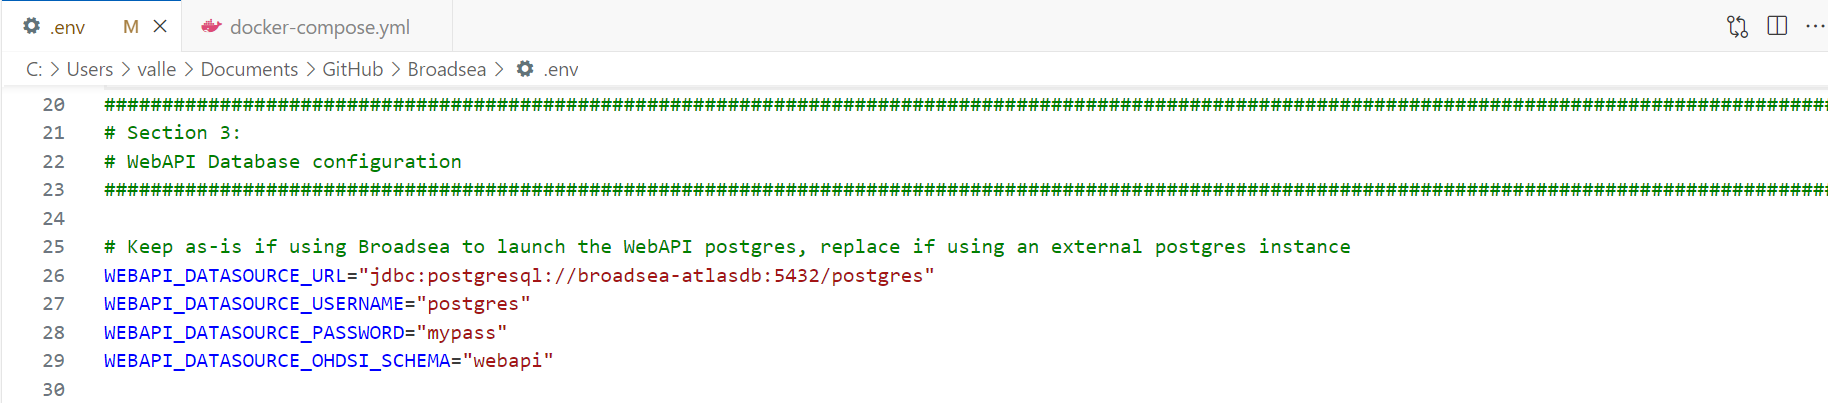
\includegraphics[width=0.90\textwidth]{figures/seccion3env.png}
     \caption{Captura de pantalla de la sección 3 del archivo \code{.env}.}
    \label{fig:seccion3env}
    \end{figure}


    Tal y como se muestra en la Figura \ref{fig:seccion3env} ''Captura de pantalla de la sección 3 del archivo \code{.env}'', en el archivo por defecto, se presenta la contraseña para acceder a la WebAPI \code{(password=mypass)} y el puerto que utiliza (\code{port=5432}).

    \item El servidor por defecto de Broadsea se solapa con el servidor local por defecto de PostgreSQL puesto que ambos se alojan en la dirección \code{127.0.0.1} y en el puerto \code{5432}. 
    
    Por tanto, para evitar este solapamiento existen varias estrategias. Una estrategia podría ser cambiar el puerto de la instancia local de Postgre para que cada instancia se aloje en espacios distintos sin solapamiento. Sin embargo, en este caso, directamente se ha detenido el servicio local de PostgreSQL, de forma que el servidor quede totalmente libre para albergar la base de datos de Broadsea.

    Para detener el servicio local de PostgreSQL lo más sencillo es abrir la aplicación \textit{servicios} buscar el servidor de postgre y deterlo, tal y como se muestra en la Figura \ref{fig:serviciosConfig} ''Captura de pantalla de la aplicación de servicios''.

    \begin{figure}[H]
    \centering
    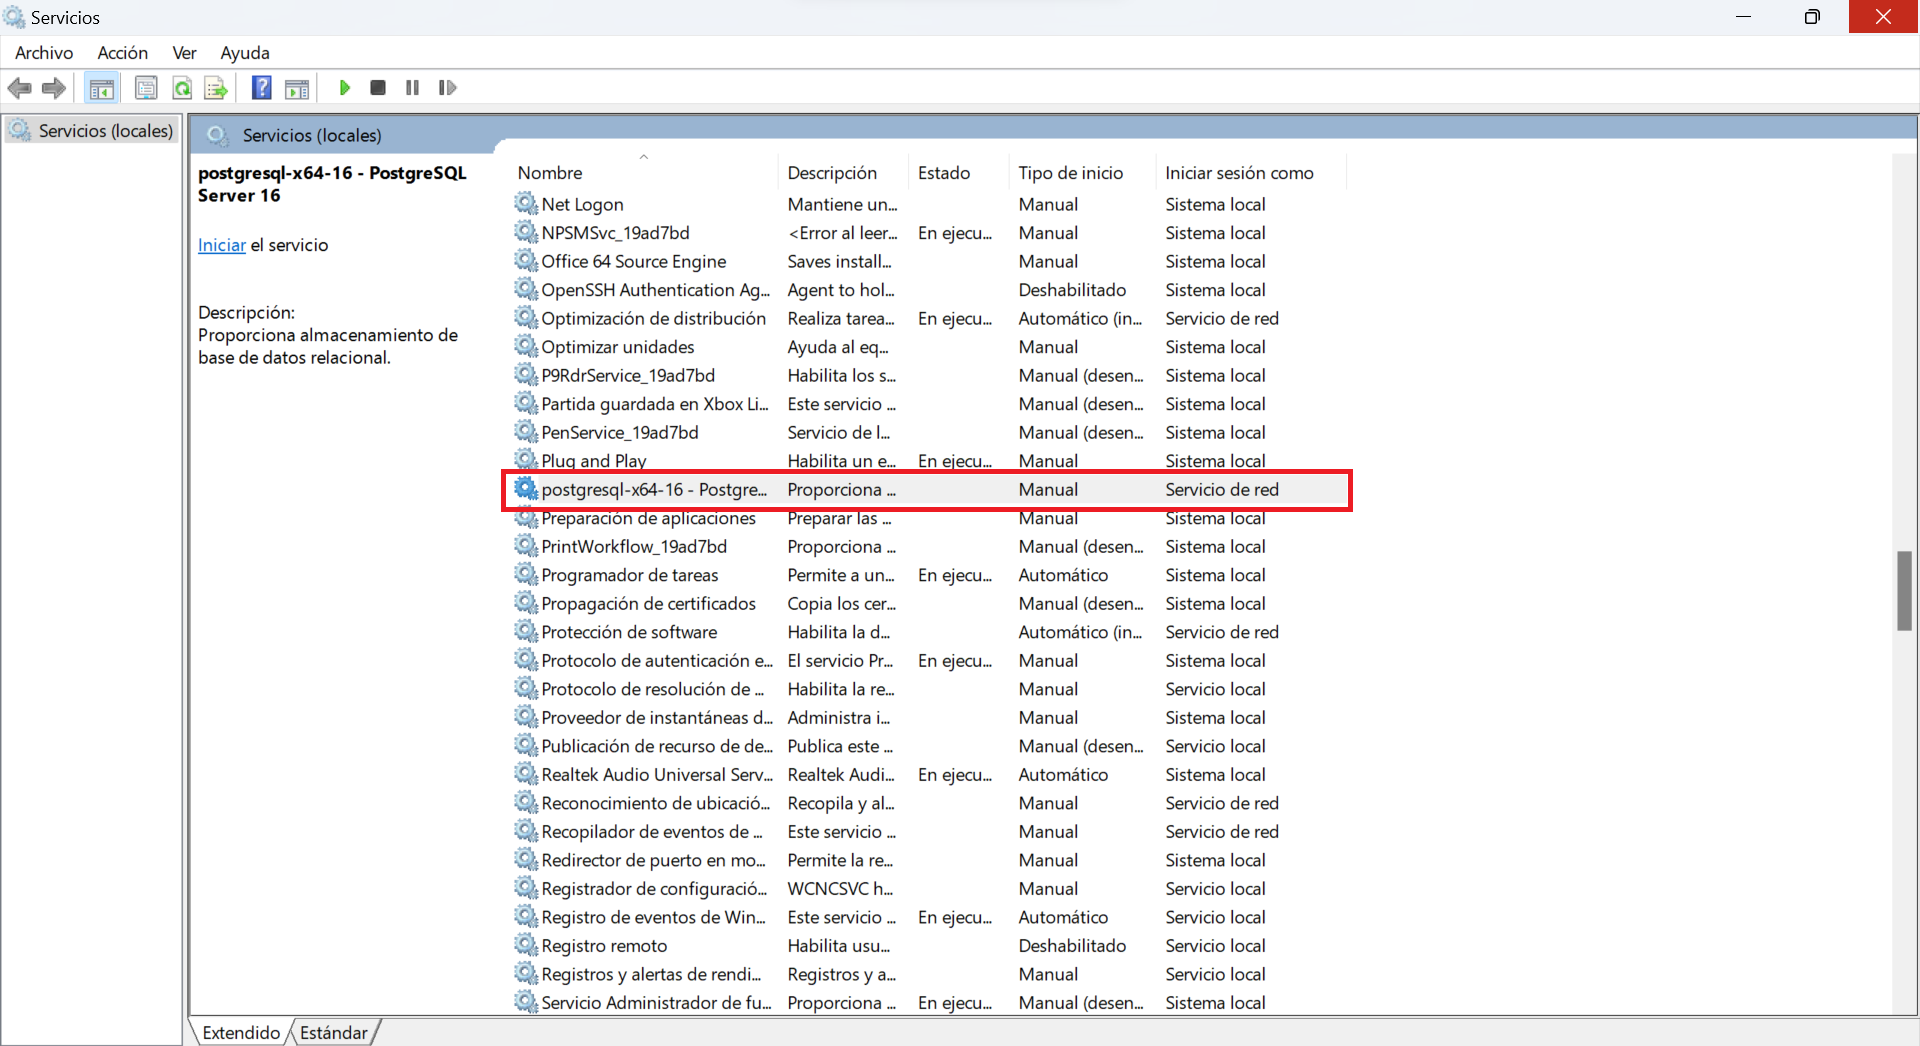
\includegraphics[width=0.90\textwidth]{figures/serviciosConfig.png}
     \caption{Captura de pantalla de la aplicación de servicios.}
    \label{fig:serviciosConfig}
    \end{figure}

    \item El último paso consiste en registrar el servidor a través del administrador de base de datos instalado en el equipo, en este caso pgAdmin. 
    
    Una vez que se haya liberado el puerto 5432, se puede registrar un nuevo servidor en dicho puerto que acceda a la base de datos de Broadsea. Para ello, abrir el administrador de la base de datos PostgreSQL, pgAdmin 4, y registrar un nuevo servidor. Los parámetros de configuración de este nuevo servidor deben ser los mismos que se establecen en la sección 3 del archivo \textit{.env}. Los parámetros fundamentales son:

    \begin{lstlisting}[language=sh]
        host = 127.0.0.1
        port = 5432
        user = postgres
        password = mypass\end{lstlisting}

    \item Tras registrar el servidor correctamente, debe aparecer una base de datos con cinco esquemas: \code{demo\_cdm}, \code{demo\_cdm\_results}, \code{public}, \code{webapi}, \code{webapi\_security} (véase \ref{sec:01Postgre} ''Entorno PostgreSQL de Broadsea'').

\end{enumerate}

\section{Comprobación de conexión correcta} \label{sec:03comprobacion}

Una vez se ha registrado el servidor de Broadsea a travñes de pgAdmin es importante comprobar que la conexión se ha realizado correctamente, sin pérdida de información. Para ello se pueden realizar distintas comprobaciones:


\begin{enumerate}[label=\alph*]

    \item \textbf{Comprobación a través de pgAdmin.} Por ejemplo, comprobar el número de filas que recupera pgAdmin de la tabla \code{person} del esquema \code{demo\_cdm}, tal y como se muestra en la Figura \ref{fig:pgAdmin} ''Captura de pantalla de pgAdmin''.

    \begin{figure}[H]
    \centering
    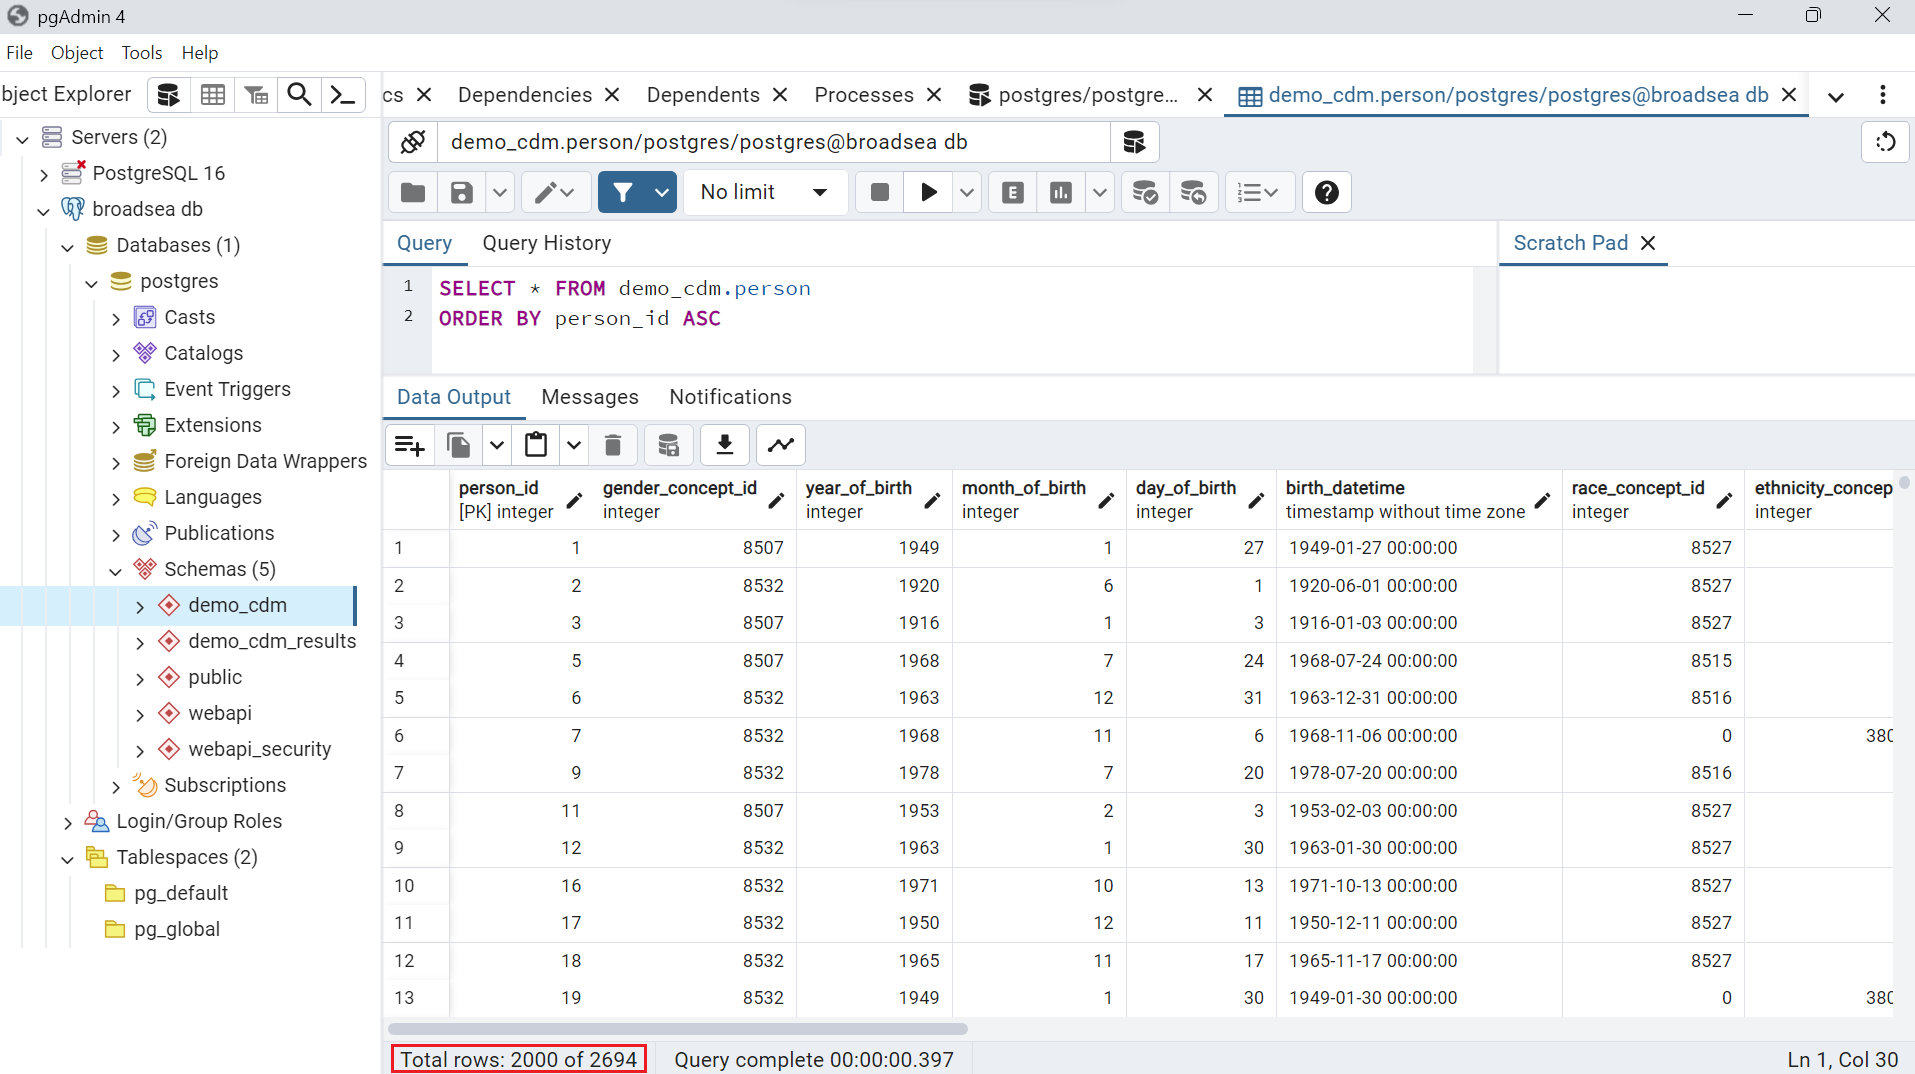
\includegraphics[width=0.90\textwidth]{figures/pgAdmin.png}
     \caption{Captura de pantalla de pgAdmin.}
    \label{fig:pgAdmin}
    \end{figure}

    El número de filas que recupere pgAdmin debe ser igual al número de personas que muestra ATLAS en la sección Data Sorce/Dashboard, en este caso son 2694 personas (Figura \ref{fig:dashboardEJ} ''Captura de pantalla de ATLAS Data Sources/Dashboard'').

    \begin{figure}[H]
    \centering
    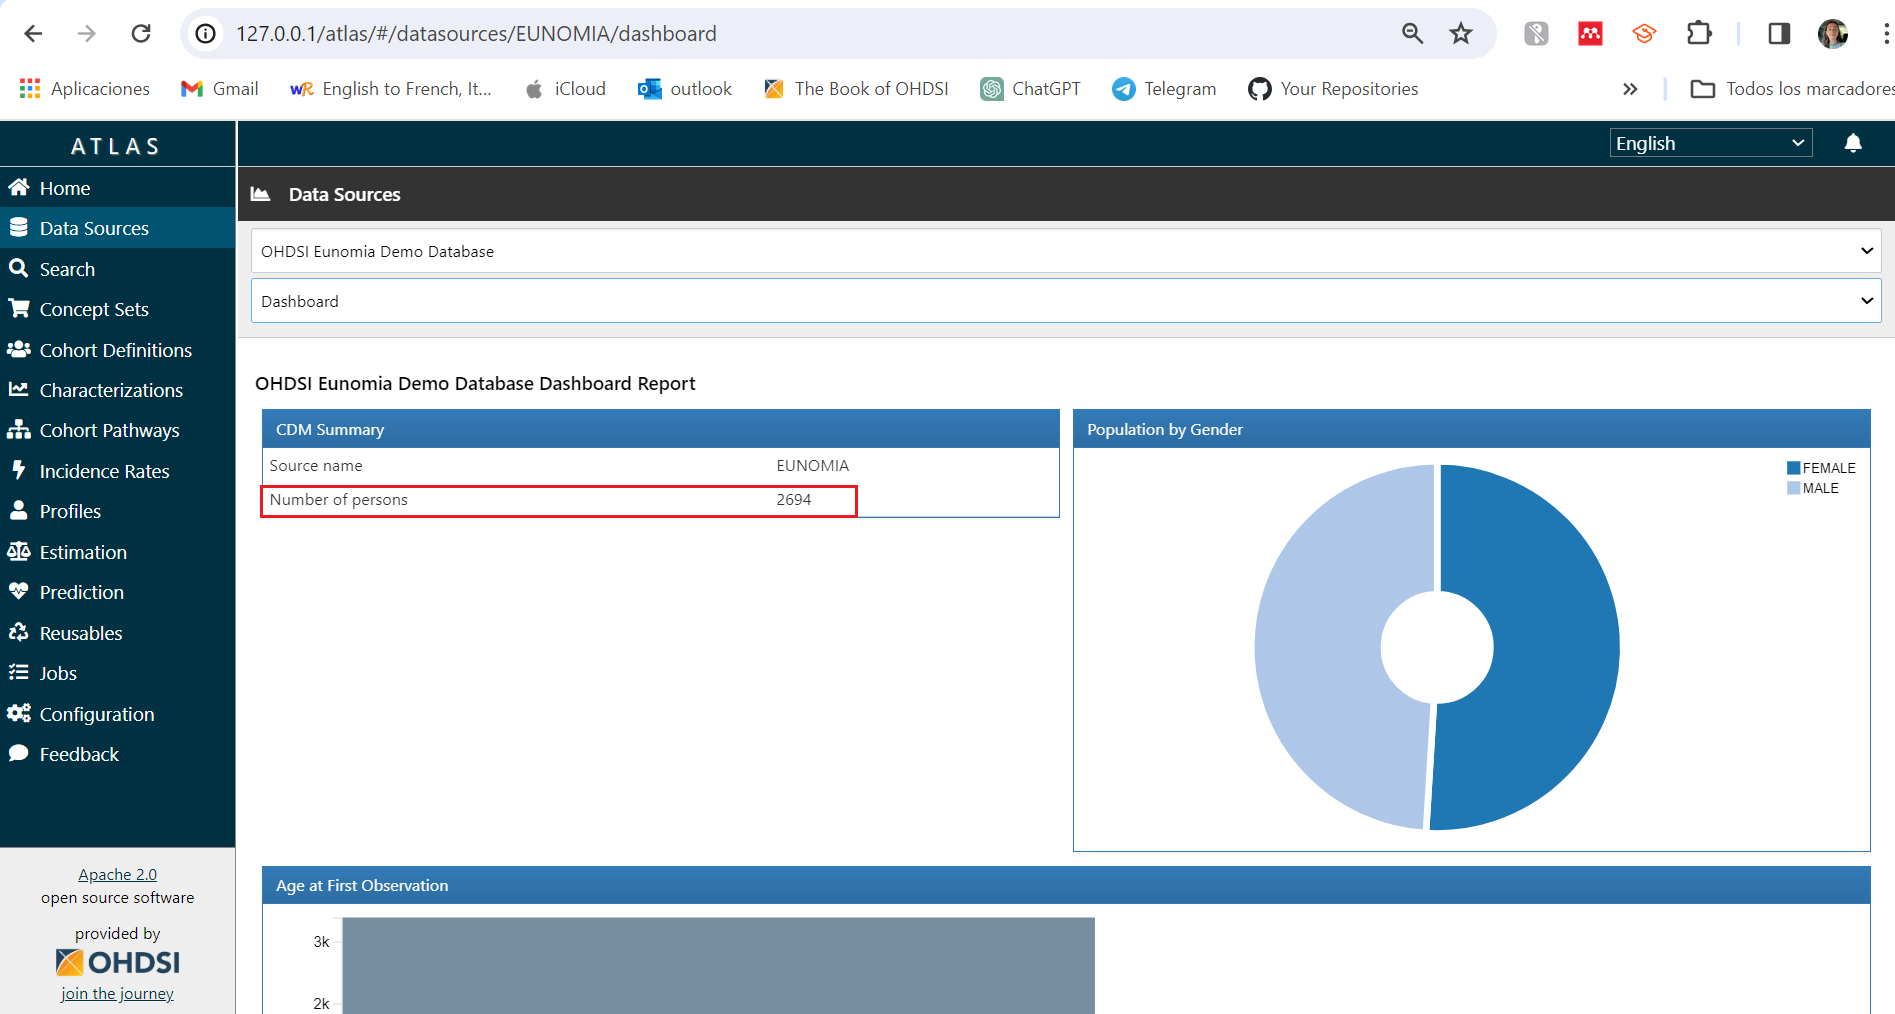
\includegraphics[width=0.90\textwidth]{figures/dashboardEJ.png}
     \caption{Captura de pantalla de ATLAS Data Sources/Dashboard.}
    \label{fig:dashboardEJ}
    \end{figure}

    \item \textbf{Comprobación a través de RStudio.} Otra forma de comprobar que la conexión es correcta y una forma alternativa de realizarla, con el fin de detectar posibles problemas durante la implementación, es ejecutar el siguiente script de código en R, que realiza la conexión con la base de datos a través de RStudio:
    
    \begin{figure}[H]
    \centering
    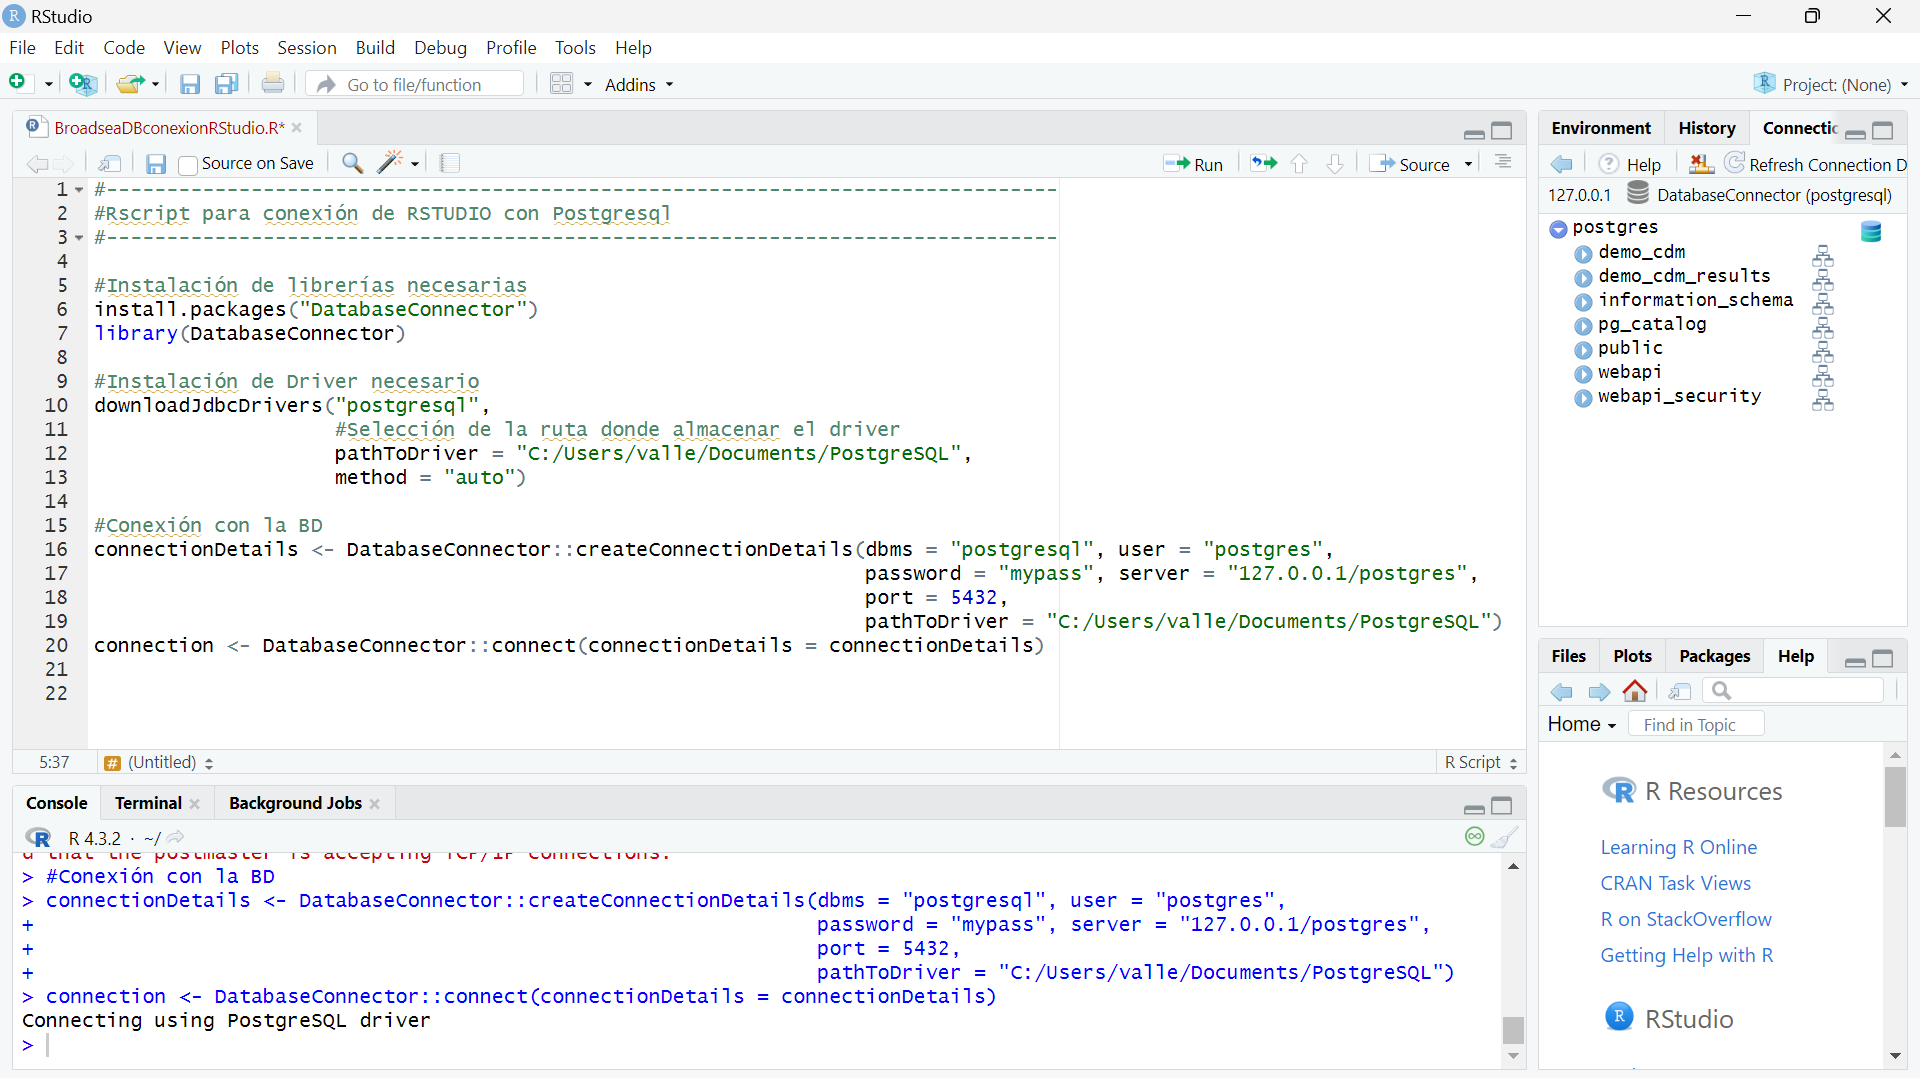
\includegraphics[width=0.90\textwidth]{figures/RStudio.png}
     \caption{Captura de pantalla de script de RStudio.}
    \label{fig:RStudio}
    \end{figure}

    El código que se muestra en la Figura está extraído (modificado) del foro \parencite{forumBroadseaDB} y está disponible en el repositorio de github del TFG en la ruta 
    \code{Thesis-ATLAS-OHDSI/files/manual/BroadseaDBconexionTest.txt} \parencite{vallealonsodc}.
    
\end{enumerate}

\section{Solución de posibles problemas} \label{sec:03problemas}

\subsubsection{Al registrar el servidor se queda pillado en ''Saving''}
Problema: A la hora de registrar el servidor por primera vez a través de pgAdmin y pulsar la opción ''save'', se mantiene cargando ''saving'' eternamente.

    \begin{figure}[H]
    \centering
    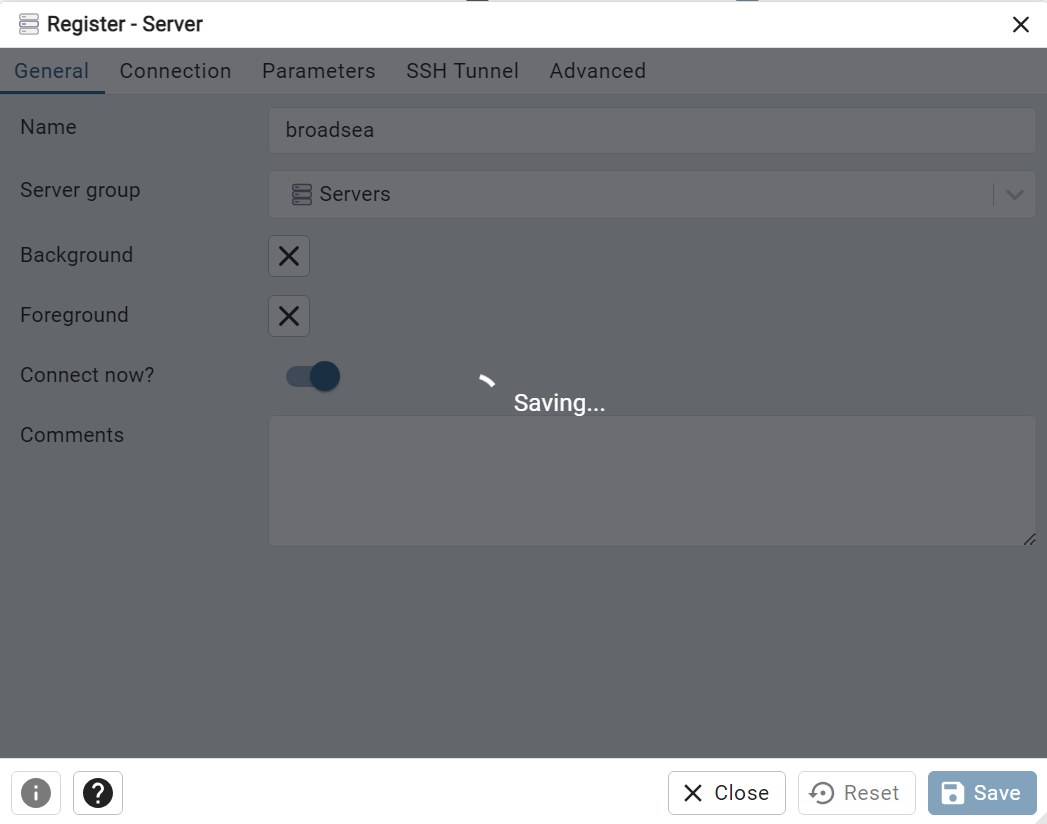
\includegraphics[width=0.70\textwidth]{figures/error03Saving.png}
     \caption{Captura de pantalla de error.}
    \label{fig:error03Saving}
    \end{figure}

Motivo: No permite registrar el servidor, probablemente porque el puerto que se pretende utilizar ya está en uso. 

Solución: Tal y como se sugiere en \ref{sec:03Deployment} ''Deployment'' o bien cambiar el puerto que utiliza la instancia local de Postgre o bien directamente detener todo el servicio local de Postgre a través de la aplicación ''Servicios''.

\subsubsection{Error: Connection timeout expired}
Problema: Al acceder al servidor de Broadsea e introducir la contraseña correctamente aparece dicho error que impide acceder al servidor.

    \begin{figure}[H]
    \centering
    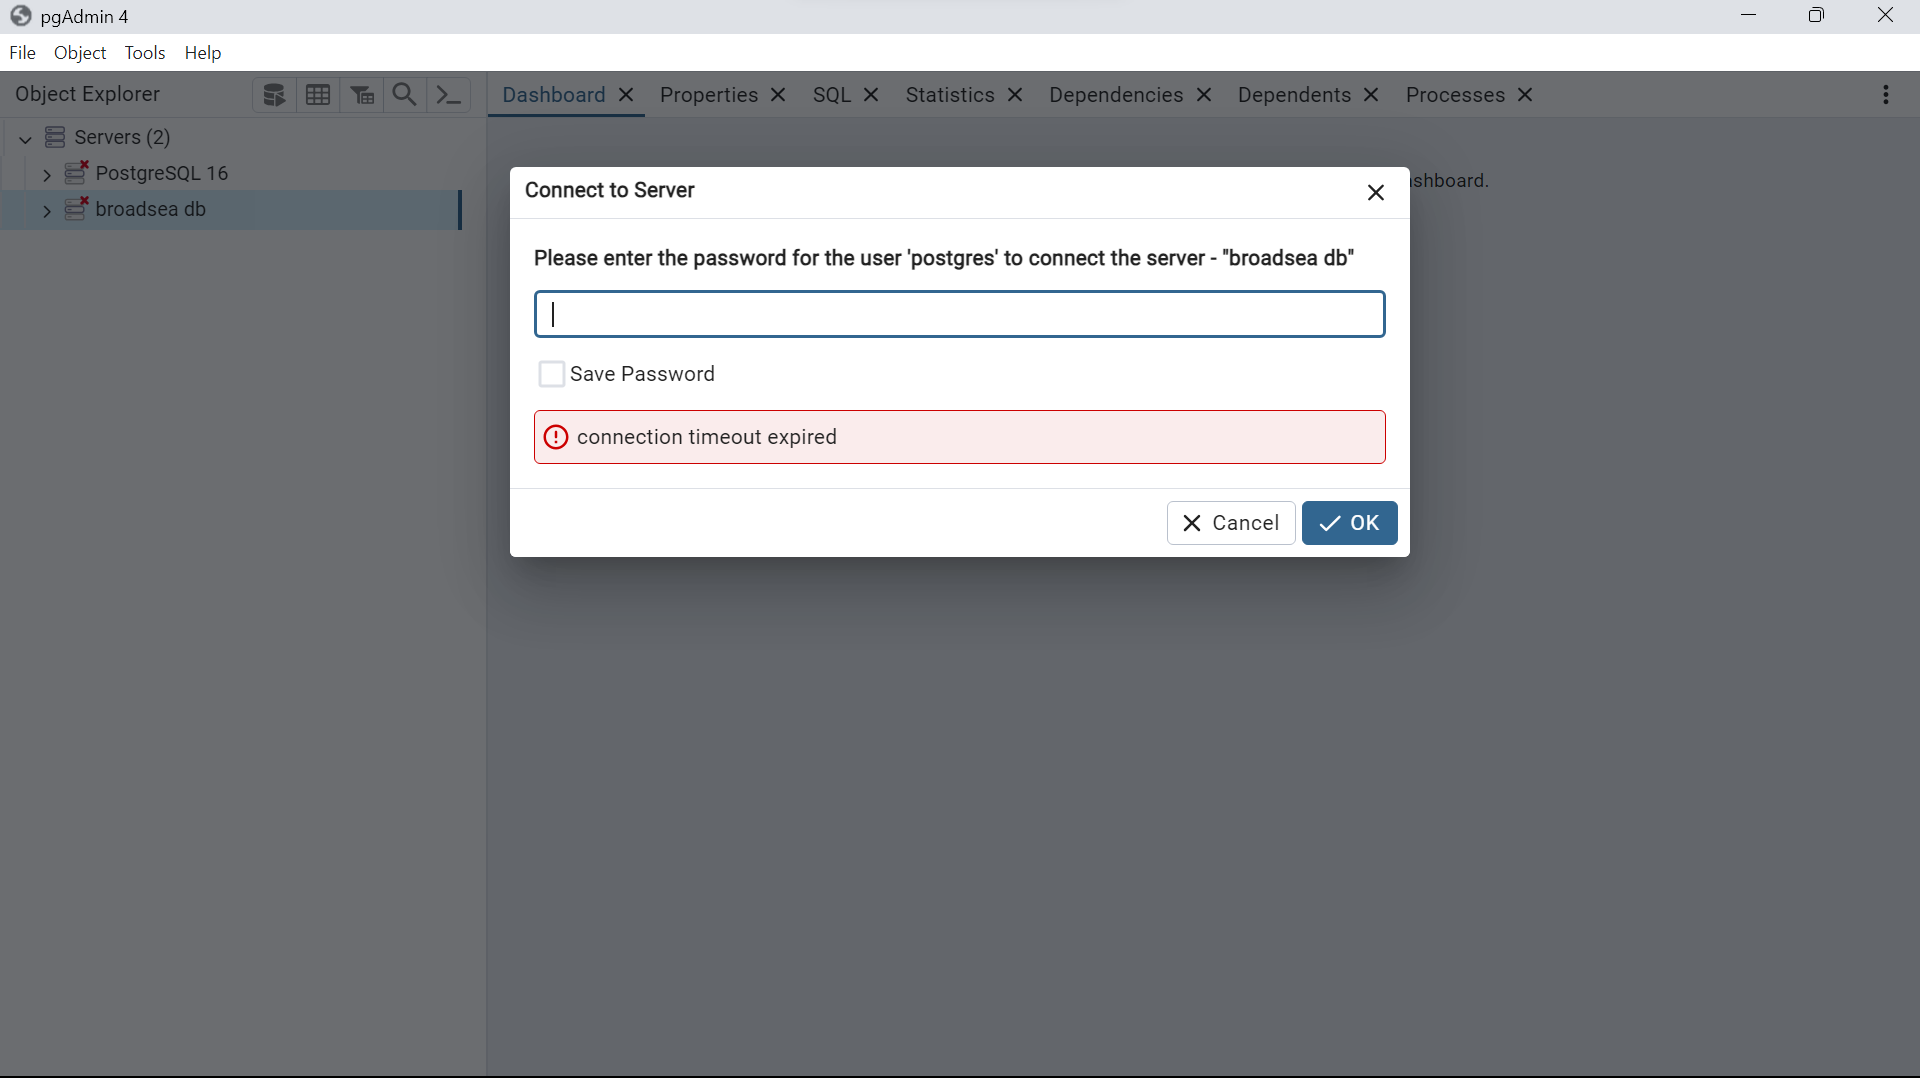
\includegraphics[width=0.90\textwidth]{figures/Error03ConnTime.png}
     \caption{Captura de pantalla de error.}
    \label{fig:Error03ConnTime}
    \end{figure}
    
Motivo: El tiempo de conexión con el servidor espira porque no se puede acceder a él porque el contenedor Docker que alberga la base de datos de Broadsea no está ejecutándose.

Solución:  Comprobar que todos los contenedores de docker implicados están corriendo, especialmente el contenedor \code{atlasdb}. Para ello acceder a Docker Desktop y ejecutar los contenedores implicados o directamente todos los pertenecientes al multicontenedor de Broadsea. 

 